\documentclass[10pt,a4paper]{scrartcl}
\usepackage[ngerman]{babel}
\usepackage[latin1]{inputenc}
%\usepackage[utf8x]{inputenc}
\usepackage[T1]{fontenc}
\usepackage{amsmath}
\usepackage{amsfonts}
\usepackage{amssymb}
\usepackage{listings}
\usepackage{pdfpages}
\usepackage{url}
\usepackage[colorlinks=true,linkcolor=black]{hyperref}
\usepackage[left=2cm,top=2cm,right=2cm,bottom=2cm]{geometry}



\begin{document}
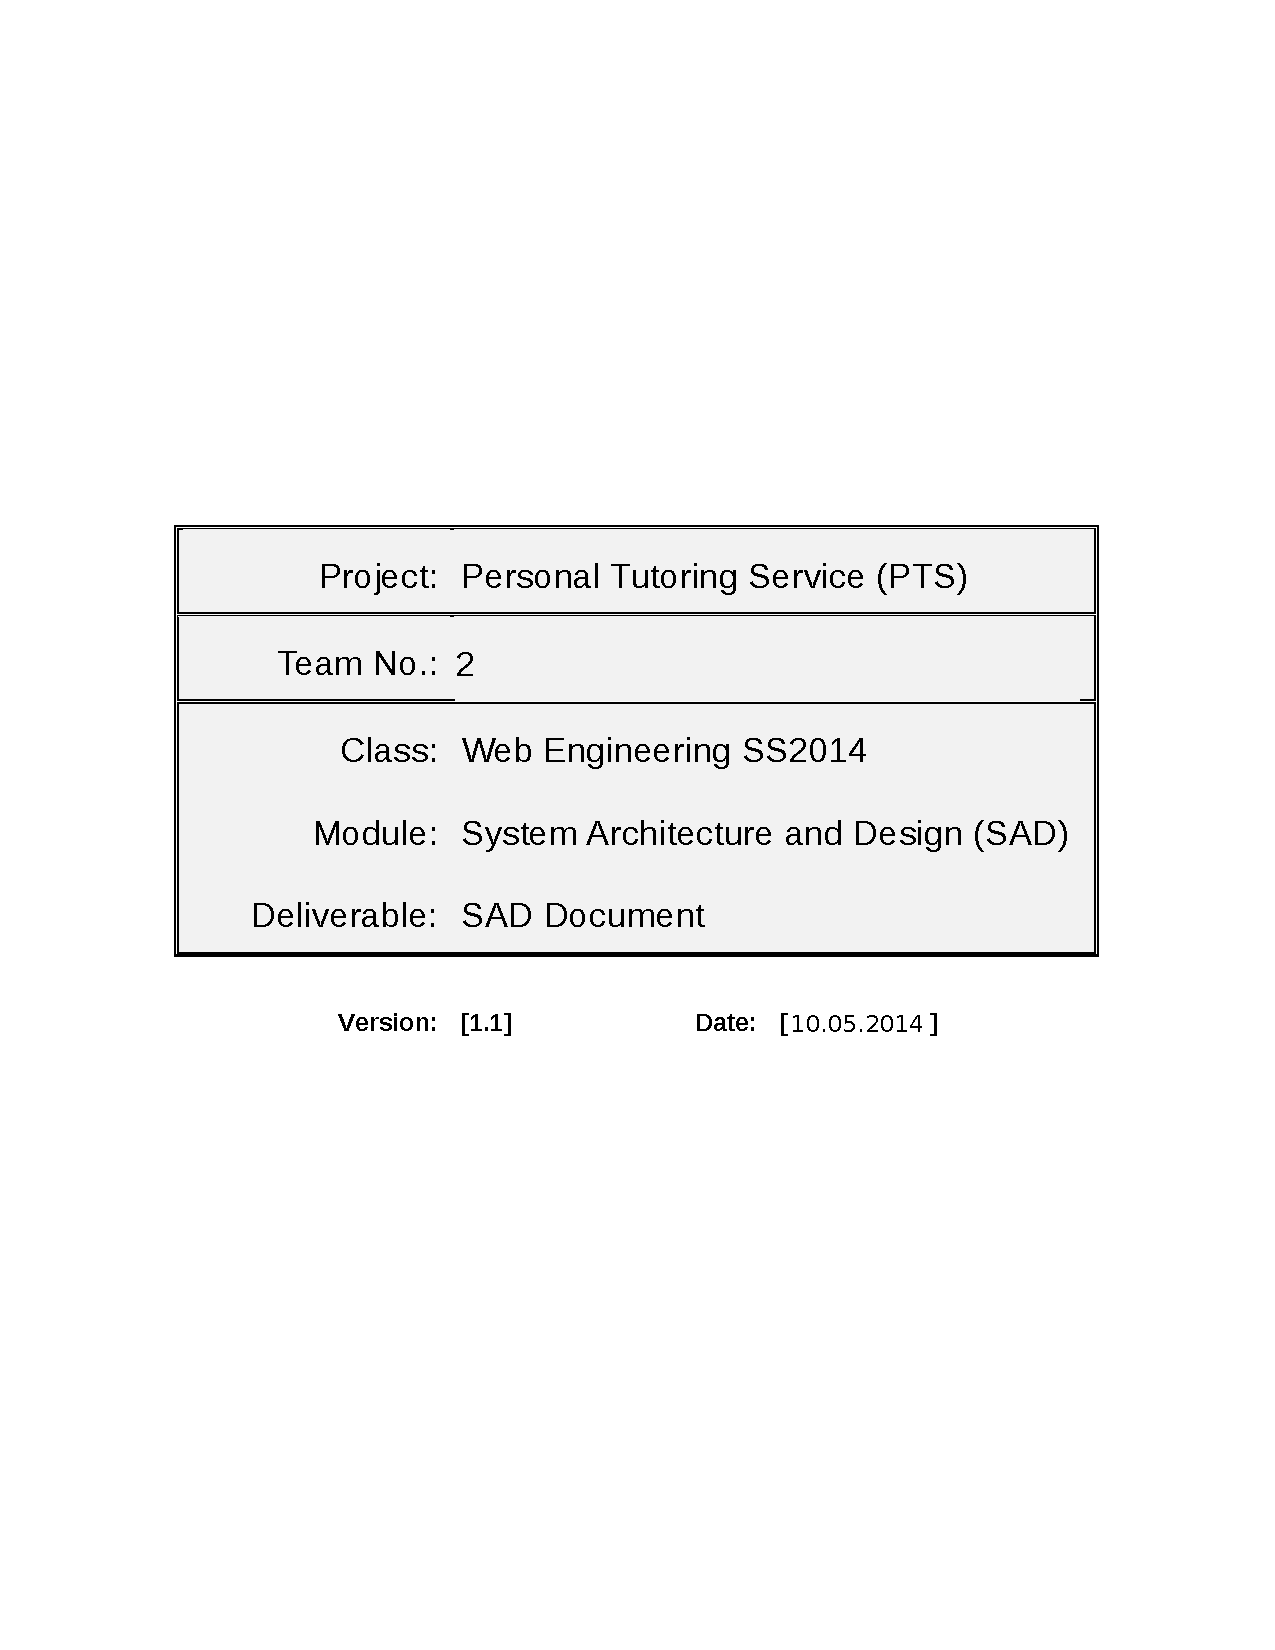
\includepdf{SAD_Titelseite.pdf}

\newpage
\begin{itemize}
\item[] \textbf{\large Beitragende:}\\
Sven Liebl\\
Matthias Goetz\\
Christian Dauerer\\
Maxmilian Schröter\\
Daniel Tatzel\\
Nils Weiss\\
Florian Laufenböck\\
Alexander Strobl\\
Matthias Birnthaler\\
Tobias Schwindl
\end{itemize}

\bigskip

\begin{table}[!h]
 	\centering
	\begin{tabular}{|c|c|c|c||p{5cm}|}
	\hline
	\textbf{VersionsNr} &  \textbf{Datum} & \textbf{Auslöser} & \textbf{Veränderungsgrad} & \textbf{Beschreibung} \\
	\hline
	1.0 & 03.05.2014 & AS & Erster Entwurf & First Draft \\
	\hline
	1.1 & 10.05.2014 & AS & Verbesserung & Missing Data added:  \newline Sequencediagram, Annahmen \\
	\hline
	1.2 & xx.06.2014 & Alle & Anpassung & \\
	\hline
	\text{ } & \text{ } & \text{ } & \text{ } & \text{ } \\
	\hline
	\end{tabular}

\caption{Überarbeitungshistorie}
\end{table}

\newpage
\tableofcontents
% \listoftables

\newpage
\section{Software Architecture}
%und alle anderen Diagramme!!

\subsection{Anwendungsfalldiagramm 1 - Administrator}
\begin{figure}[!htbp]
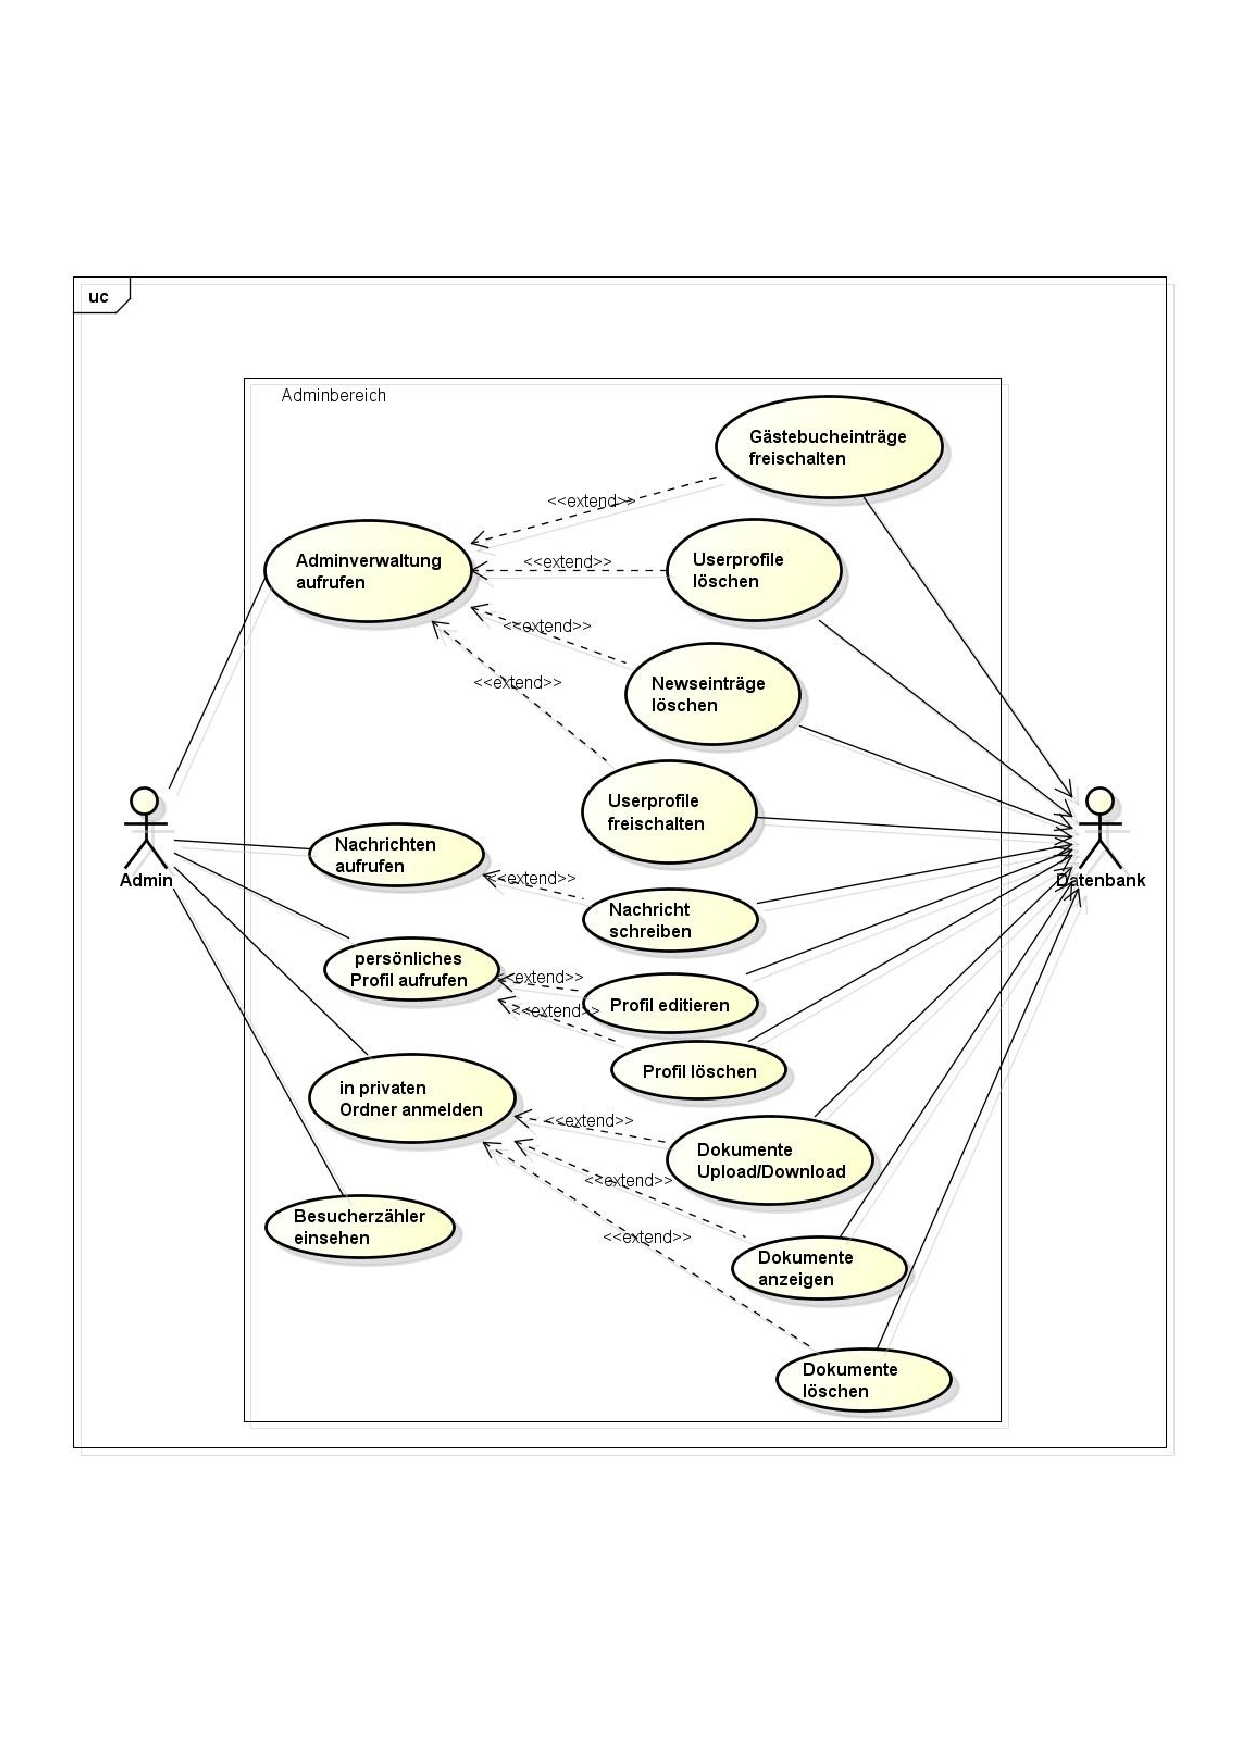
\includegraphics[width=0.8\textwidth]{./Source/UseCaseAdministrator_11.pdf}
\caption{Dieses Anwendungsfalldiagramm beschreibt die Funktionen, die ein eingeloggter Administrator ausführen kann. Des Weiteren sind die Funktionen auf einzelne Unterfunktionen aufgeschlüsselt.}
\end{figure}
\newpage
\subsection{Anwendungsfalldiagramm 2 - Tutor}
\begin{figure}[!htbp]
\fbox{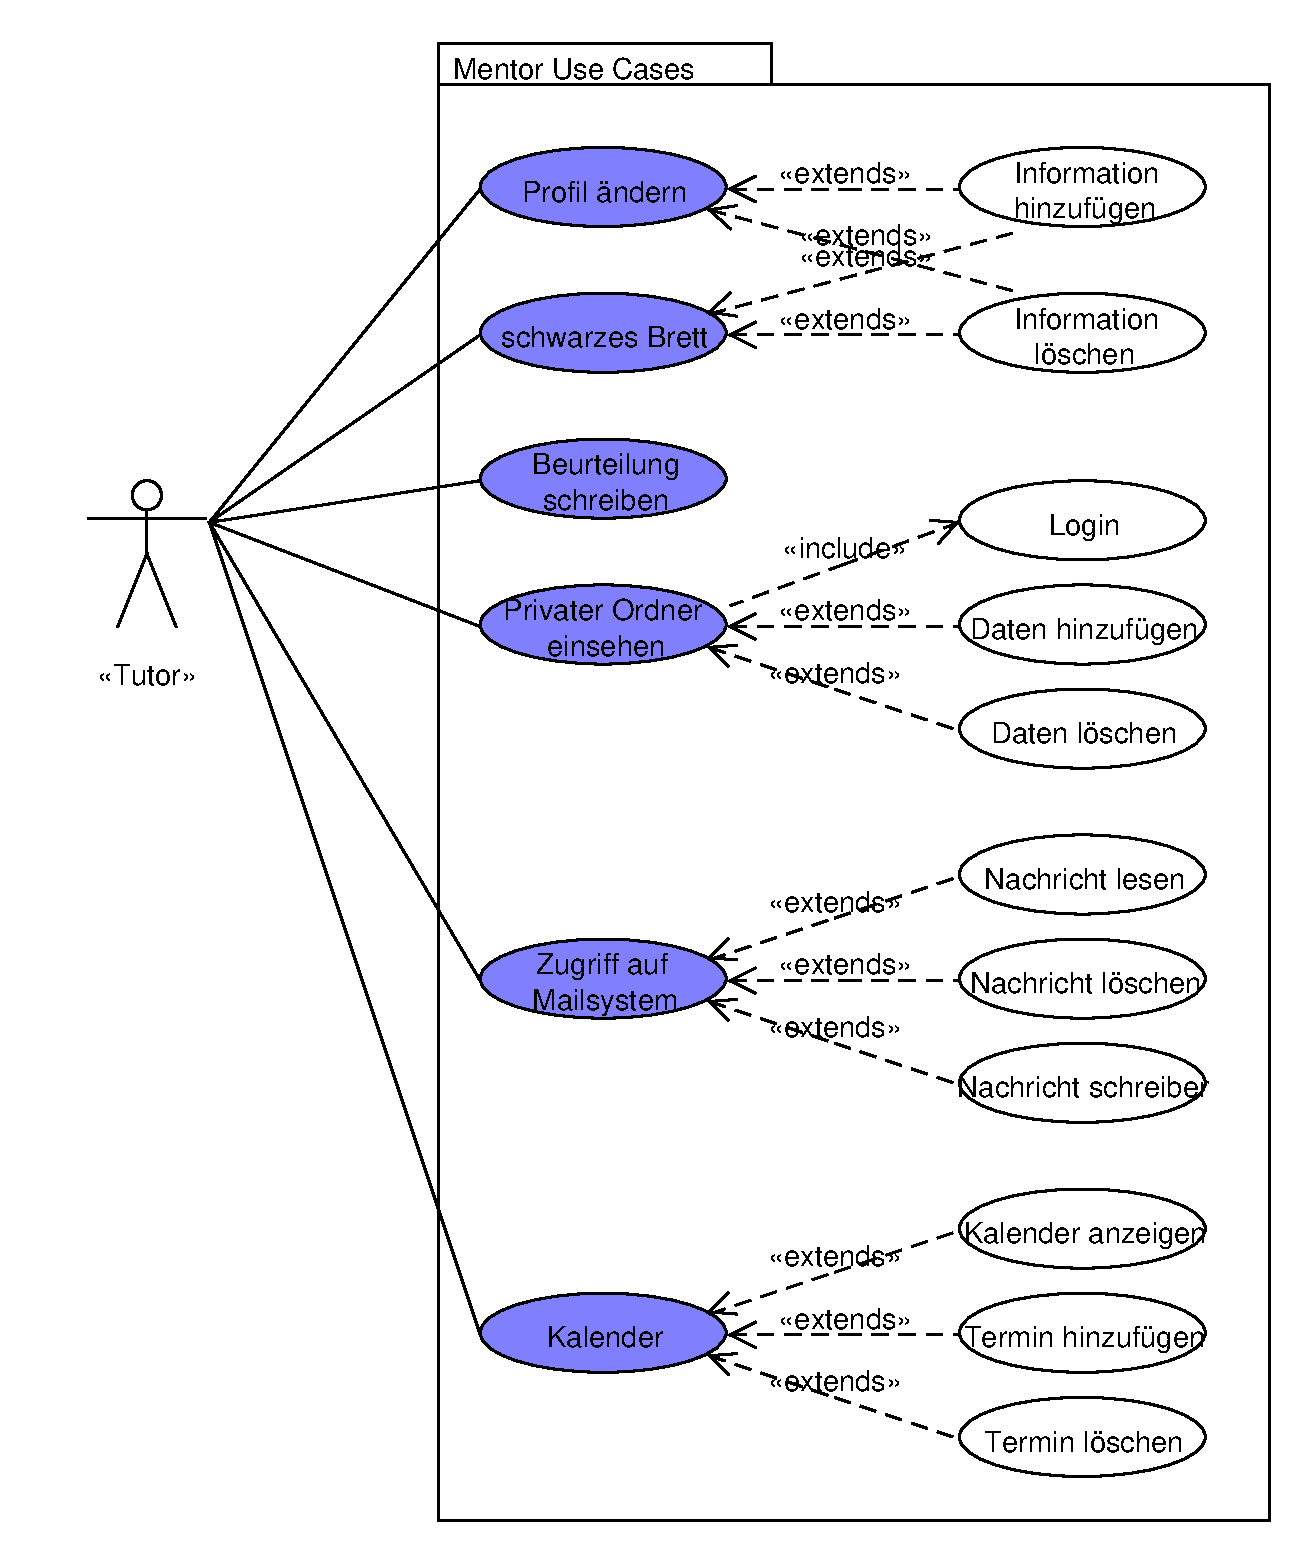
\includegraphics[width=0.9\textwidth]{./Source/UseCaseMentor_13.pdf}} \caption{Dieses Anwendungsfalldiagramm beschreibt die Funktionen, die ein eingeloggter Tutor ausführen kann. Des Weiteren sind die Funktionen auf einzelne Unterfunktionen aufgeschlüsselt.}
\end{figure}
\newpage
\subsection{Sequenzdiagramm}
\begin{figure}[!htbp]
\fbox{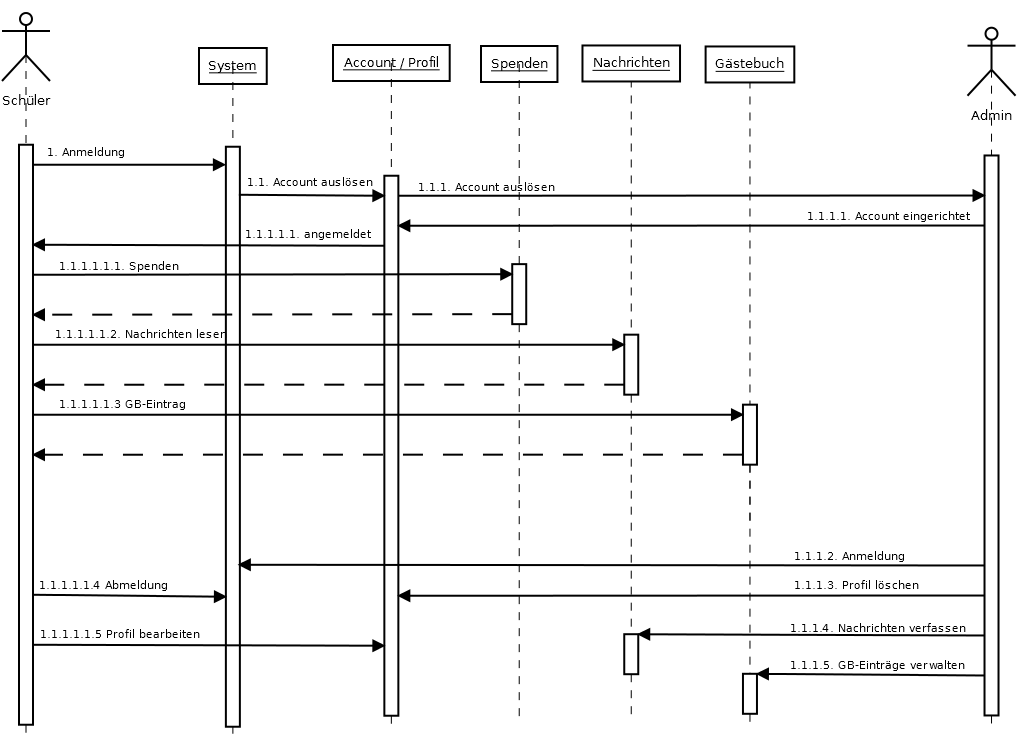
\includegraphics[width=0.9\textheight, angle=-90]{./Source/sequence_diagram.png}}
\caption{Dieses Sequenzdiagramm beschreibt, in welcher Reihenfolge Befehle ausgeführt werden müssen, um eine Aktion vollständig und korrekt auszuführen}
\end{figure}
\newpage
\subsection{Navigationdiagramm}
\begin{figure}[!htbp]
\fbox{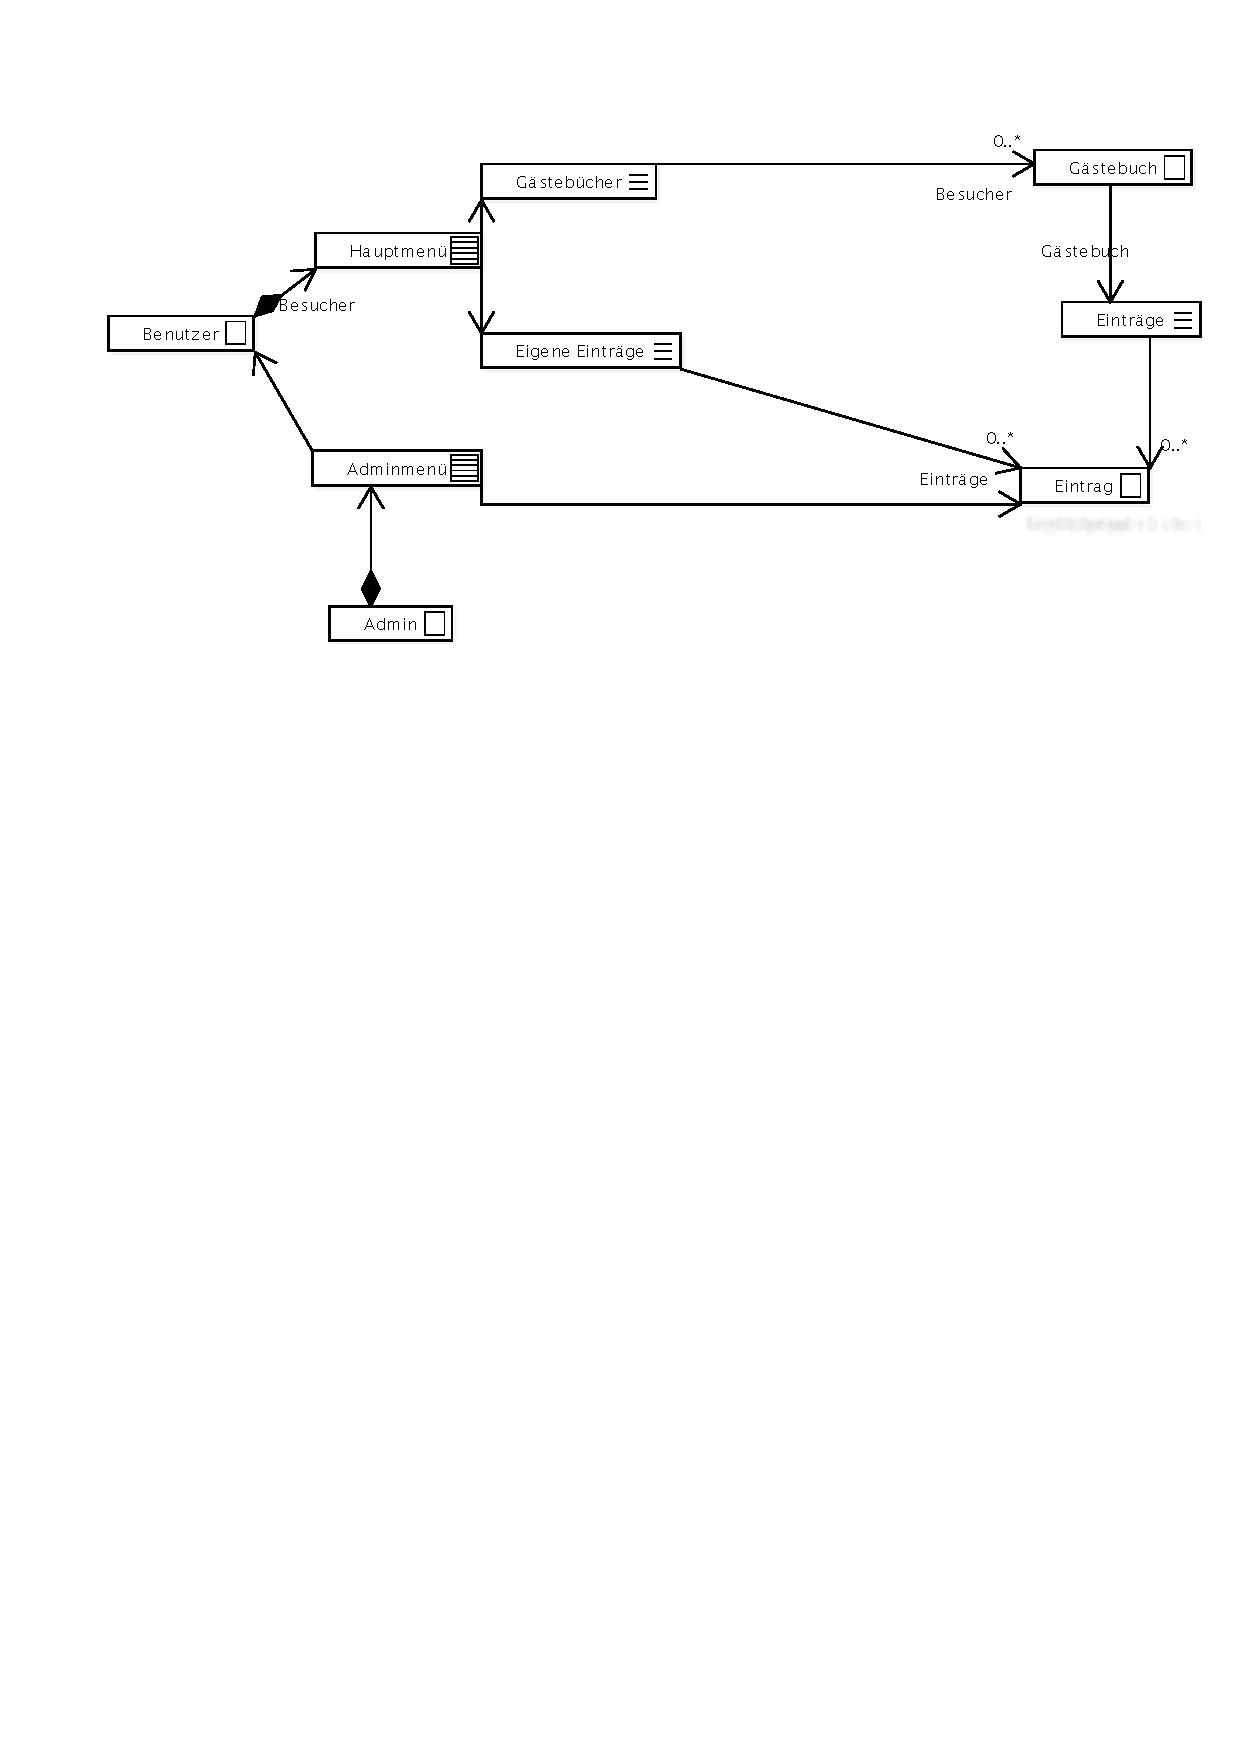
\includegraphics[width=0.9\textwidth]{./Source/navigation_diagram.pdf}} \caption{Dieses Navigationdiagramm beschreibt die Menüführung für ein Gästebuch und Gästebucheinträge. Es wird zwischen einem Menü für normale Besucher und Administratoren unterschieden. Ausserdem ist eine Navigation zu einem Gästebuch oder zu allen erstellten Einträgen eines Benutzers vorgesehen.}
\end{figure}
\newpage
\subsection{ER-Diagramm}
\begin{figure}[!htbp]
\fbox{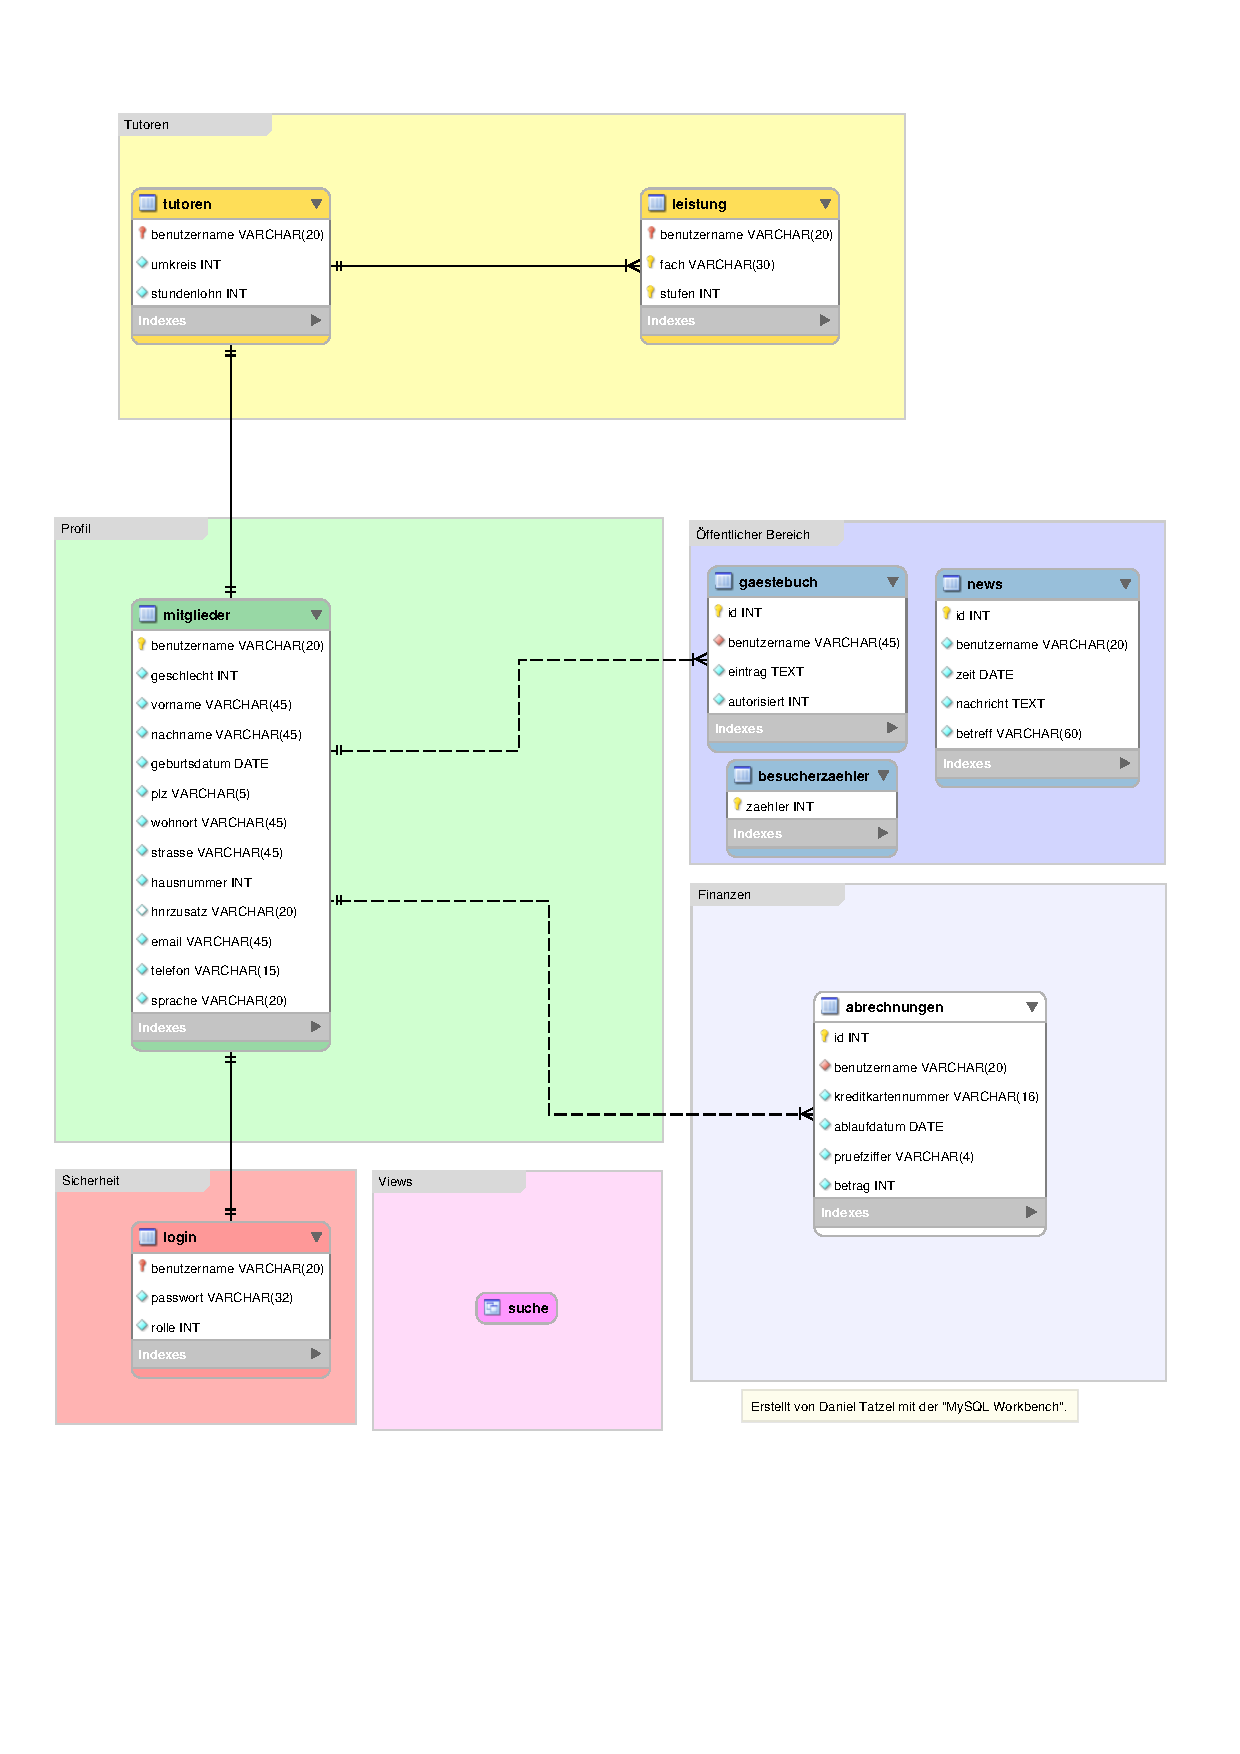
\includegraphics[width=0.9\textwidth,page=1]{../../DB/ER-Diagramm.pdf}} \caption{Entity-Relation Diagramm der Datenbank}
\end{figure}
\newpage
\subsection{Activitydiagramm}
%Viet, Stefan
\begin{figure}[!htbp]
\fbox{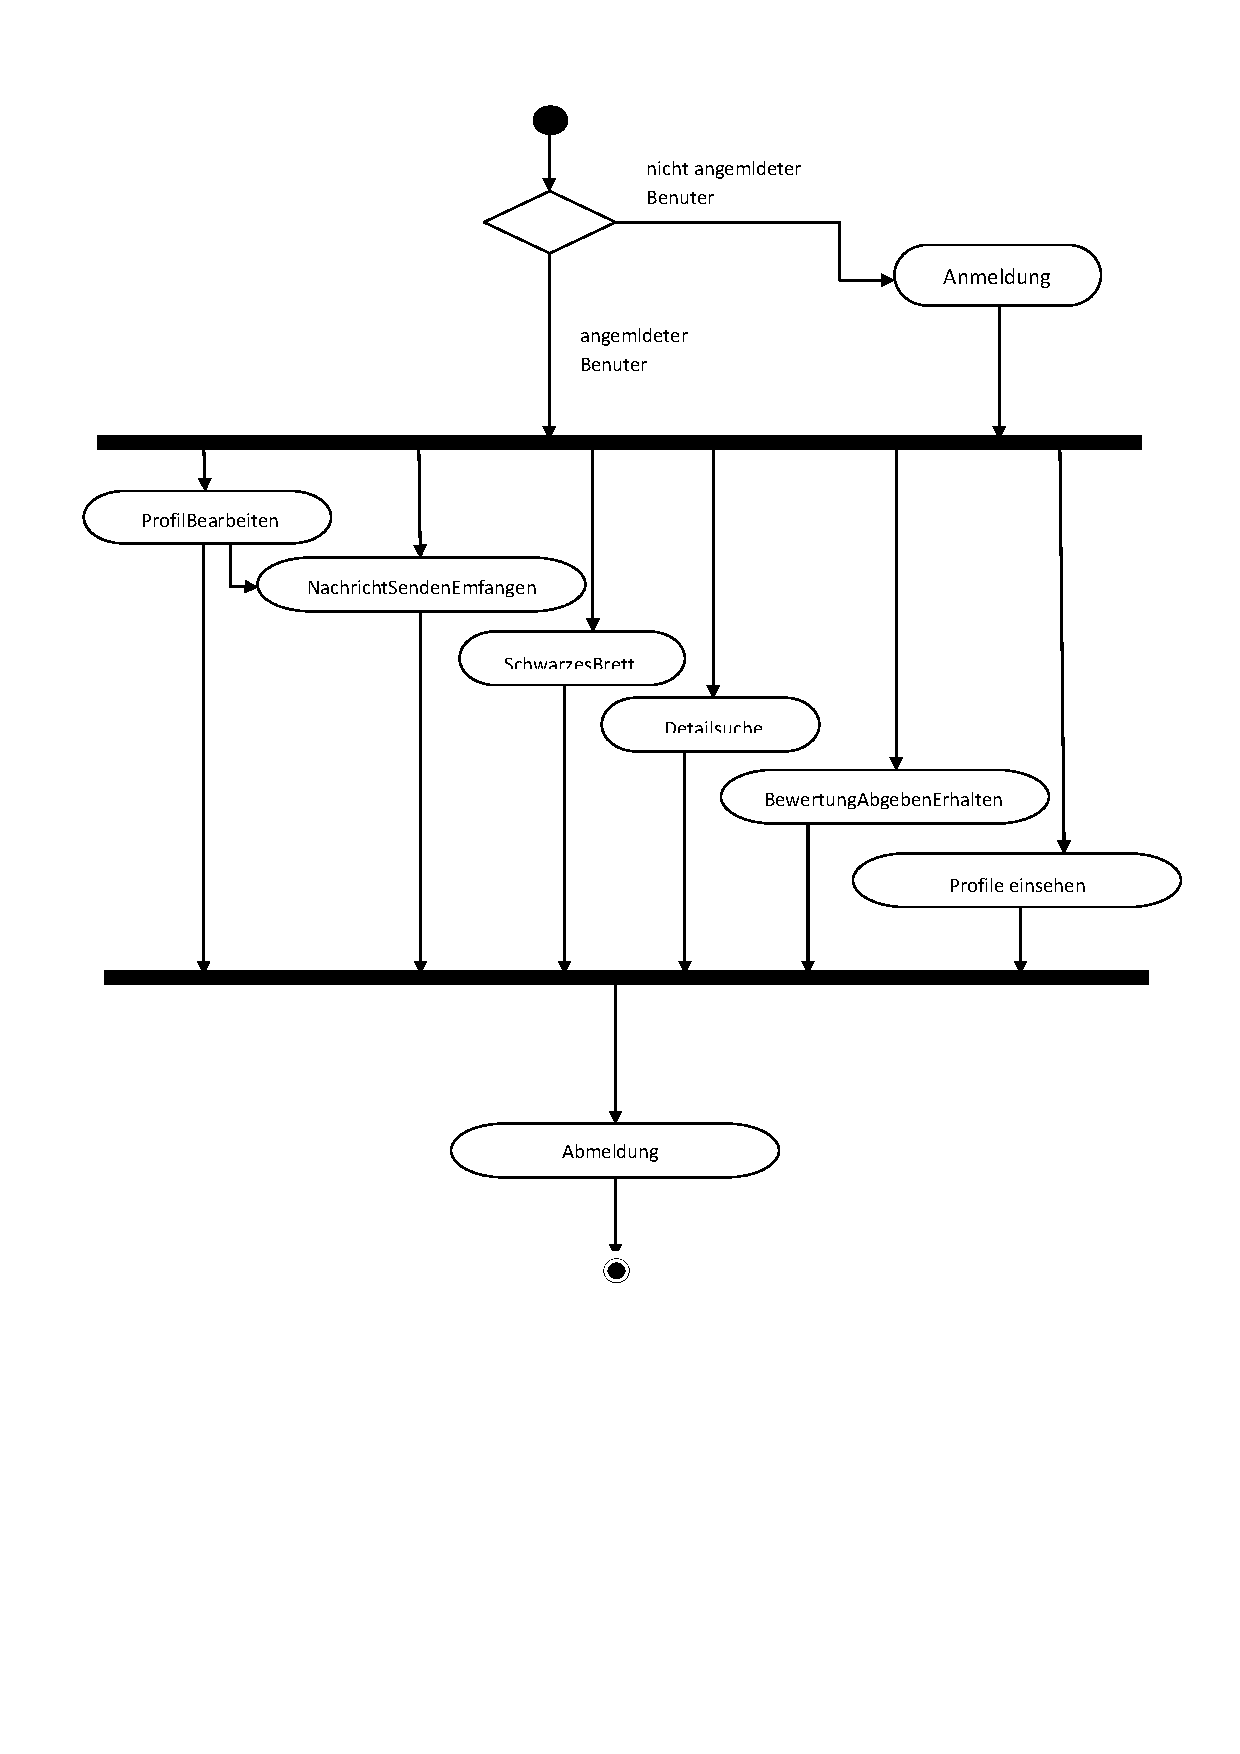
\includegraphics[width=0.9\textwidth]{./Source/ActivityNew.pdf}}
\caption{User muss sich anmelden, um die erweiterten Funktionen nutzen zu können. Bei erfolgreicher Anmeldung hat der User die Möglichkeit folgende Aktivitäten zu nutzen: Profil bearbeiten, Nachrichten senden und empfangen, Zugriff auf das Schwarze Brett, erweiterte Detailsuche, Bewertung erhalten und abgeben und in Profile einsehen. Um den persönlichen Bereich wieder zu verlassen, muss der User sich abmelden. }
\end{figure}
\newpage
\section{Objectives}

\subsection{Business Objectives}
Ziel der Webseite ist es Tutoren in der Nähe zu finden, und mit Ihnen in Verbindung zu treten. Durch die Möglichkeit ein persönliches Profil erstellen zu können, sollen Nutzer dauerhaft an unser Webangebot gebunden werden. Potentielle Nutzer sollen direkt an Hochschulen geworben werden. Auch Kooperationen mit Universitäten und Hochschulen sollen geschlossen werden.
\newline \newline
Unser Webangebot soll kostenfrei sein. Finanziert werden soll das Angebot durch gezielte Werbung.

\subsection{System Objectives}
Das Webangebot Personal Tutoring Service soll als `Template` aufgebaut werden.
Somit soll es möglich sein, leicht andere Vermittlungsportale, wie z.B. eine
Mitfahrzentrale aufzubauen. Somit sollen sich mit geringem Aufwand schnell neue
Geschäftszweige erschliessen lassen.

\section{Systems Requirement}

\subsection{F1: Öffentlicher Bereich}
\subsubsection*{F11: Startseite}
%Matthias G. und Sven
Informiert den Besucher über das Auswahlkonzept bzw. $-$kriterien der Tutoren. Ebenfalls wird eine Karte mit den Standorten von Tutoren in Deutschland implementiert. Ein Teaser über das Motto und der Angebote der Website soll den Besucher ansprechen und so sein Interesse fördern. Durch die Anzeige von Top Gästebucheinträgen wird dem Gast das Gefühl der Vertrauenswürdigkeit und der Kompetenz übermittelt.
\newline \newline
\textbf{Karte}\newline
Es wird eine Karte von Google-Maps eingebettet. Dies funktioniert mit Hilfe des bereitgestellten Iframes von Google.
\newline \newline
\textbf{Slideshow}\newline
Die Bilder der Slideshow werden mit HTML5 zur Verfügung gestellt. Mittels CSS3 werden die Bilder formatiert. JQuery sorgt für die Slideanimation.
\newline \newline
\textbf{Video}\newline
Das Video wird mit HTML5 implementiert und ist dadurch ohne Flash abspielbar. Die Kontrollfunktionen werden ebenfalls mit HTML5 zur Verfügung gestellt. Gesteuert wird der HTML5 Videoplayer mit JavaScript.
\newline \newline
\textbf{Top Gästebucheinträge}\newline
Nach dem Laden der Seite wird eine Javascript-Funktion ausgeführt, welche die Top-Gästebucheinträge über ein Json-Objekt erhält. Diese Einträge werden über JQuery eingeblendet und über CSS3 formatiert.

\subsubsection*{F12: Gästebuch}

Das Gästebuch ermöglicht den Nutzern eigene Kommentare abzugeben. Diese werden in einer SQL - Datenbank abgespeichert. Zusätzlich wird dazu der Autor abgespeichert und eine Variable, welche erfasst, ob ein Gästebuch eintragt bereits von einem Administrator autorisiert wurde, oder nicht. Mittels PHP, im speziellen mit dem PDO werden die Gästebucheinträge zum Frontend der Website weitergeleitet und dort angezeigt. Einträge, die sehr gute Bewertungen erhalten werden zur Werbung für die Website eingesetzt.

\subsubsection*{F13: Anzeige von verfügbaren Tutoren an einem bestimmten Ort}

Die Wohnort-Tutorensuche wird mit Hilfe von JavaScript und MySQL umgesetzt. Benutzer gibt einen Ort oder ein Fach ein und die Datenbank wird nach Eintr\"agen von Tutoren mit identischem Ort oder Fach durchsucht und die Anzahl der Eintr\"age wird anschlie{\ss}end zur\"ukkgegeben. 
Suchvorschläge erhält der Nutzer unmittelbar während der Suche, sobald mehr als 
2 Zeichen eingegeben wurden. 
% \subsubsection*{F14: Erweiterte Suchkriterien}
%
% Die Suche wird mittels einer View realisiert. Diese View enthält alles notwendigen Informationen, die es dem User ermöglichen das gewünschte Suchergebnis zu finden,
% \begin{itemize}
%  \item Benutzername
%  \item Wohnort
%  \item Umkreis
%  \item Stundenlohn
%  \item Bewertung
%  \item Fächer
%  \item Stufen
% \end{itemize}
%
% Die View wird verwendet um in den normalen Tabellen keine Redundanzen zu haben.

\subsubsection*{F14: Registrierungs- und Anmeldefenster}

Die Registrierung erfolgt über ein Formular, in der alle Daten, die unbedingt notwendig sind, ausgefüllt werden müssen. Das Onlineformular ist im \underline{HTML5}-standard geschrieben, um gleich Validierungen der Eingaben durchführen zu können, ohne die Informationen erst zum Server schicken zu müssen. Zus\"atzlich werden die Eingaben per Javascript \"uberpr\"uft. Wenn alle Daten eingegeben wurden, die Validierungen erfolgreich waren, klickt der Benutzer auf einen Button und schickt die Daten damit zum Server. Dort wird der Benutzername \"uberpr\"uft und falls dieser noch nicht vorhanden ist, dann werden die Daten mittels \underline{PHP} zur \underline{Datenbank} geschickt, um dort gespeichert zu werden. Der Aufruf des Scripts zum Eintragen der Informationen in die Datenbank wird mittels JQuery ausgef\"uhrt.
\bigskip
\newline
Ist ein Nutzer registriert, so kann er sich über die Login-Maske, die auf jeder Seite eingebunden ist, anmelden. Hierfür wird eine Datenbank Abfrage mittels PHP und SQL über PDO generiert um die Identität des Nutzers zu prüfen. Bei erfolgreicher Authentifizierung der Benutzerdaten werden mehrere Sesseion-Variablen, die angeben, dass der Benutzer angemeldet ist und um welchen Benutzer es sich handelt, initialisiert um immer entsprechende Informationen über den Benutzer zu haben. Das Script zum Anmelden wird ebenfalls per JQuery aufgerufen.

\subsubsection*{F15: About us (Impressum)}

%Alex
Hierbei handelt es sich um statischen Inhalt für den HTML als Formatierung des Textes benutzt wird. Erreichbar ist das Impressum über einen Link in der Navigationsleiste.

% \subsubsection*{F16: Preismodell und Zahlungsinfos}
%
% %Alex
% Hierbei handelt es sich um statischen Inhalt für den HTML als Formatierung des Textes benutzt wird. Erreichbar ist Preismodell und Zahlungsinfos über einen Link in der Navigationsleiste.

\subsubsection*{F16: Auswahl der Sprache}

Jeder Besucher bekommt eine \underline{Serverseitige Sessionvariable}, in der die Sprache gespeichert wird. Im Kopf einer jeden Seite wird diese Variable mit der Sprache der aktuellen Seite definiert. Diese Variable wird im weiteren Verlauf der Seite genutzt um in den entsprechenden Bereichen wie in der "`Navigation"' genutzt um die Inhalte der entsprechenden Sprache zu laden. Dies wird nur f\"ur die Elemente genutzt, die auf jeder Seite eingebunden werden. Jede Seite besitzt eine "`Dummy-Datei"' in der der entsprechende Inhalt geladen wird. Diese "`Dummy-Datei"' wird f\"ur entsprechende \"Uberpr\"ufungen und f\"ur das ausf\"uhren von Scripten benutzt.

Wechselt ein Benutzer die Sprache, dann wird er mithilfe von RewriteRules in einer htaccess Datei auf die entsprechende Seite der jeweils anderen Sprache geleitet. Es befindet sich eine htaccess Datei mit entsprechenden RewriteRules in den jeweiligen Ordner f\"ur die Sprachen.  \underline{PHP} pr\"uft zur Laufzeit welche Sprache gesetzt ist und l\"adt die entsprechende Sprache f\"ur das Template.

\subsubsection*{F17: Support und Kontaktdaten}

%Alex
Der Benutzer erfährt hier die Kontaktdaten des Supports, an den er sich bei Fragen und Problemfällen wenden kann. Hierbei handelt es sich um statischen Inhalt für den HTML als Formatierung des Textes benutzt wird. Erreichbar ist das Impressum über einen Link in der Navigationsleiste.


\subsection{F2: Administrator}
\subsubsection*{F21: Anmelden}

Der Administrator kann sich über die Login-Maske, die auf jeder Seite eingebunden ist, anmelden. Hierfür wird eine Datenbank Abfrage mittels PHP und SQL über PDO generiert um die Identität des Administrator zu prüfen. Bei erfolgreicher Authentifizierung der Benutzerdaten werden mehrere Session-Variablen, die angeben, dass der Administrator angemeldet ist und um welchen Benutzer es sich handelt, initialisiert um immer entsprechende Informationen über den Benutzer zu haben. Danach hat der Administrator erweiterte Zugriffsrechte um ihm die Verwaltung zu erleichtern. Der Aufruf des Scripts zum Anmelden wird mittels JQuery ausgef\"uhrt.

\subsubsection*{F22: Persönliche Einstellungen}

%Matthias G und Sven
Der Admin kann durch Ausfüllen von HTML5 Formularen seine Profildaten bearbeiten. Die Eingabe des Users wird mittels HTML5 und JavaScript überprüft. Die Daten in der Datenbank werden über ein PHP Skript geändert.

\subsubsection*{F23: Bearbeiten von Kundenkonten$^1$ und Kundeninformationen$^2$}

Ist ein Nutzer als Administrator eingeloggt, hat dieser die Möglichkeit sich eine Übersicht aller Kundenkonten anzeigen zu lassen. Diese Informationen werden in Form einer Tabelle auf
einer separaten Seite angezeigt. Beim Aufruf der Seite werden alle notwendigen Informationen
über Ajax aus der Datenbank geladen und über JSON an den Browser des Admins geliefert. Um
bei einer grossen Datenbank die Wartezeit gering zu halten, werden die Daten nur teilweise
aus der Datenbank geladen. So ist es beispielsweise nicht sinnvoll mehr wie 20 Datensätze
gleichzeitig zu laden, da in der Regel nicht mehr angezeigt werden kann.
\newline \newline
Durch eine Tabellen-PlugIn für jQuery werden die Rohdaten übersichtlich dargestellt.
Die Tabelle soll ausserdem die Möglichkeit bieten die Datensätze nach Spalten zu sortieren.
\newline \newline
Änderungen der Daten werden ebenfalls über jQuery an die Datenbank übergeben, wenn der Administrator
einen "Speichern" Knopf drückt.
\newline \newline
Die Validierung der Daten wird über HTML5 und gegebenenfalls mit einer PHP-Funktion durchgeführt.

% \subsubsection*{F24: Zugriff auf Nachrichtensystem}
%
% In der Datenbank befinden sich eine grosse Tabelle in der alle Nachrichten als Rohdaten abgelegt werden.
% Jeder Datensatz hat die Felder: Absender, Empfänger, Datum, Zeit, Nachricht, gelesen.
% Über SQL-Abfragen werden die jeweiligen Nachrichten aus der Datenbank geladen und über JSON an ein
% jQuery-Script übergeben. Möchte ein Nutzer Beispielsweise alle gesendeten Nachrichten einsehen, wird
% der aktuell angemeldete Nutzername in die \textit{"WHERE"}-Klausel der Datenbankabfrage eingefügt, um so nur
% die relevanten Nachrichten abzufragen.
% \newline \newline
% Zum Abrufen der Nachrichten wird dem angemeldeten Nutzer eine spezielle Webseite zur Verfügung gestellt,
% auf welcher er Nachrichten abrufen und erstellen kann. Die Anzeige wird in Form einer Tabelle über
% ein jQuery-Plugin erstellt.
% \newline \newline
% Zum Versenden von Nachrichten muss ein Nutzer den Benutzernamen eines Empfängers in ein Textfeld eingeben.
% Bevor eine Nachricht abgesendet werden kann, erfolgt eine Validierung des Benutzernamens des Empfängers.
% Diese Validierung wird durch ein Javascript vorgenommen.
% Für das Eingabefeld des Empfängers ist es denkbar eine Autovervollständigung über Ajax zur Verfügung zu stellen.

\subsubsection*{F24: Freischaltung von Gästebucheinträge}

Der Administrator ruft das Gästebuch auf und sieht alle nicht autorisierten Einträge. Diese kann er autorisieren. Dann werden diese in der Datenbank aktualisiert.

\subsubsection*{F25: Abmelden}

Jeder angemeldete Nutzer kann sich auch wieder abmelden, dies geschieht durch löschen einer Session-Variable, die bei der erfolgreichen Anmeldung gesetzt wurde. Das löschen der Variable hat keinen Einfluss auf die restlichen Inhalte der Session.

\subsubsection*{F26: Besucherzähler}

Jeder Aufruf der Startseite wird über eine enstprechende Zählvariable, die in der Datenbank gespeichert ist, mitprotokolliert. Hierfür wird beim Aufbau der Startseite der aktuelle Zählerstand in der Datenbank um eins erhöht, dies geschieht mittels PHP und PDO zum Ansprechen der Datenbank.
\bigskip
\newline
$^1$ Kundenkonten: Tutorenkonten und Schülerkonten\\
$^2$ Kundeninformationen: Persönliche Informationen der Kundenkonten

\subsection{F3: Schüler}
Jeder Besucher hat die Möglichkeit ein Profil anzulegen und sich mit den erhaltenen Zugangsdaten einzuloggen.
Dadurch erhält er Zugriff auf seinen Privaten Bereich, in dem er seine bei der Registrierung hinterlegten persönlichen Daten ändern kann.
Die persönlichen Daten setzen sich aus Vorname, Nachname, Alter, Anschrift, Passwort und Kontaktdaten zusammen.
Es besteht die Option seinen Account zu löschen.

% \subsubsection*{F31: Detaillierte Suche}
%
% Die Suche wird mittels einer View realisiert. Diese View enthält alles notwendigen Informationen, die es dem User ermöglichen das gewünschte Suchergebnis zu finden,
% \begin{itemize}
%  \item Benutzername
%  \item Wohnort
%  \item Umkreis
%  \item Stundenlohn
%  \item Bewertung
%  \item Fächer
%  \item Stufen
% \end{itemize}
%
% Die View wird verwendet um in den normalen Tabellen keine Redundanzen zu haben.

\subsubsection*{F31: Sch\"ulerprofil}

%Matthias G und Sven
Der Schüler kann durch Ausfüllen von HTML5 Formularen seine Profildaten bearbeiten. Die Eingabe des Users wird mittels HTML5 und JavaScript überprüft. Die Daten in der Datenbank werden über ein PHP Skript geändert.


\subsubsection*{F32: Tutorenprofil}


Der angemeldete Benutzer ist in der Lage die Profile von anderen einzusehen.

% \subsubsection*{F34: Zugriff auf Nachrichtensystem}
%
% In der Datenbank befinden sich eine grosse Tabelle in der alle Nachrichten als Rohdaten abgelegt werden.
% Jeder Datensatz hat die Felder: Absender, Empfänger, Datum, Zeit, Nachricht, gelesen.
% Über SQL-Abfragen werden die jeweiligen Nachrichten aus der Datenbank geladen und über JSON an ein
% jQuery-Script übergeben. Möchte ein Nutzer Beispielsweise alle gesendeten Nachrichten einsehen, wird
% der aktuell angemeldete Nutzername in die \textit{"WHERE"}-Klausel der Datenbankabfrage eingefügt, um so nur
% die relevanten Nachrichten abzufragen.
% \newline \newline
% Zum Abrufen der Nachrichten wird dem angemeldeten Nutzer eine spezielle Webseite zur Verfügung gestellt,
% auf welcher er Nachrichten abrufen und erstellen kann. Die Anzeige wird in Form einer Tabelle über
% ein jQuery-Plugin erstellt.
% \newline \newline
% Zum Versenden von Nachrichten muss ein Nutzer den Benutzernamen eines Empfängers in ein Textfeld eingeben.
% Bevor eine Nachricht abgesendet werden kann, erfolgt eine Validierung des Benutzernamens des Empfängers.
% Diese Validierung wird durch ein Javascript vorgenommen.
% Für das Eingabefeld des Empfängers ist es denkbar eine Autovervollständigung über Ajax zur Verfügung zu stellen.

\subsection{F4: Lehrer / Mentor}
\subsubsection*{F41 Profil einstellen}

%Matthias G und Sven
% Weiter ausführen, mit Kursen usw
Der Tutor kann durch Ausfüllen von HTML5 Formularen seine Profildaten bearbeiten. Die Eingabe des Users wird mittels HTML5 und JavaScript überprüft. Die Daten in der Datenbank werden über ein PHP Skript geändert.

% \subsubsection*{F42 Lehrmaterialien online stellen und verteilen}
%
% Jeder Schüler muss sich in Online-Kurse eintragen, bei welchem Tutor er welches Fach belegt. Der Tutor kann über einen Upload-Bereich(jquery bietet diese Möglichkeit) Dateien zum Server laden, dort werden diese in der \underline{Datenbank} gespeichert.
% Der Schüler kann sich dann die Formulare über den Browser wieder herunterladen
%
% \subsubsection*{F43 Beurteilungen schreiben}
%
% Stefan und Viet
%
% Der Schüler kann Feedback für seine abgegeben Aufgaben / Leistungen erhalten

% \subsubsection*{F42 Schwarzes Brett}
%
% Das Schwarze Brett wird mit JavaScript und MySQL umgesetzt. Die Ank\"undigungen werden in die Datenbank geschrieben und k\"onnen von dort abgerufen werden.


% \subsubsection*{F43: Zugriff auf Nachrichtensystem}
%
% In der Datenbank befinden sich eine grosse Tabelle in der alle Nachrichten als Rohdaten abgelegt werden.
% Jeder Datensatz hat die Felder: Absender, Empfänger, Datum, Zeit, Nachricht, gelesen.
% Über SQL-Abfragen werden die jeweiligen Nachrichten aus der Datenbank geladen und über JSON an ein
% jQuery-Script übergeben. Möchte ein Nutzer Beispielsweise alle gesendeten Nachrichten einsehen, wird
% der aktuell angemeldete Nutzername in die \textit{"WHERE"}-Klausel der Datenbankabfrage eingefügt, um so nur
% die relevanten Nachrichten abzufragen.
% \newline \newline
% Zum Abrufen der Nachrichten wird dem angemeldeten Nutzer eine spezielle Webseite zur Verfügung gestellt,
% auf welcher er Nachrichten abrufen und erstellen kann. Die Anzeige wird in Form einer Tabelle über
% ein jQuery-Plugin erstellt.
% \newline \newline
% Zum Versenden von Nachrichten muss ein Nutzer den Benutzernamen eines Empfängers in ein Textfeld eingeben.
% Bevor eine Nachricht abgesendet werden kann, erfolgt eine Validierung des Benutzernamens des Empfängers.
% Diese Validierung wird durch ein Javascript vorgenommen.
% Für das Eingabefeld des Empfängers ist es denkbar eine Autovervollständigung über Ajax zur Verfügung zu stellen.

\subsection{F5: Registrierte Benutzer}

\subsubsection*{F51: Spenden per Kreditkarten}

Ein registrierter Benutzer kann per Kreditkarte Spenden. Dazu gibt er seine Kreditkarteninformationen in ein HTML5 Formular Kreditkartennummer, Ablaufdatum der Karte, die Prüfziffer und den zu zahlenden Betrag. Diese werden mit Javascript auf Richtigkeit der Informationen geprüft (HTML5 Formular) und dann für die weitere Verwendung in der MySQL Datenbank gespeichert.

\section{Annahmen und Beschränkungen}
\subsection{Annahmen}

\subsubsection*{Zahlungsverkehr}
Wir nehmen an, dass alle unsere Besucher über ein Mindestalter von 14 Jahre verfügen, um so keine gesonderten rechtlichen Bestimmungen für den Zahlungsverkehr erfüllen zu müssen.
Wir führen keine Bezahlvorgänge durch, sondern vermitteln diese nur zwischen den jeweiligen Vertragspartnern. Diese führen die Bezahlvorgänge über externe Dienstleister durch.
Die weiteren Bestimmungen des Vertrages bleiben hiervon unberührt.

\subsubsection*{Mindestalter}
Das Mindestalter für die Vermittlung auf unserer Webseite beträgt 14 Jahre.


\subsection{Beschränkungen}

\subsubsection*{Leistung}

Einer der wichtigsten Dinge, auf die zu achten ist, ist die Kommunikation zwischen \underline{Javascript} und \underline{PHP}
über \underline{AJAX}. Wenn man mit Hilfe von Javascript Daten dynamisch über PHP bzw. PDO aus einer Datenbank laden will, sollte man
sehr genau auf die Performance dieses Prozesses achten. Wenn man *.php Skripte ansteuert, sollte man in diesen darauf achten, dass
das Skript an sich sehr performant ist(z.B. nicht viele, große Klassenobjekte generieren, Operationen durchführen die sehr lange brauchen,
wie z.B. aufwendige Hash-Operationen), da sonst die Datengenerierung im PHP-Skript sehr lange dauert und dies dazu führt, dass
es relativ lange dauert, bis aktualisierte Informationen auf dem Bildschirm des End-Users angezeigt werden.
\newline \newline
Um diesem Umstand gerecht zu werden, sollen die Files so angelegt werden, dass pro File möglichst wenig Funktionen enthalten sind.
Damit soll ein möglichst hoher Grad an Unabhängigkeit von anderen Funktionen erreicht werden, sodass in jedem *.php File nur die
für die darin enthaltenen Funktionen benötigten Komponenten ausgeführt werden müssen.

\subsubsection*{PHP Funktionen aus Javascript}

Da man mit Hilfe Javascript nur einzelne *.php-Skripte ansprechen kann und nicht einzelne Funktionen aus php wird es für die meisten Javascript-Funktionen eine *.php-Datei geben, die die Dinge ausführt, die Serverseitig gemacht werden sollen. Damit kann man auch mehrere serverseitige Methoden auf ein Mal abarbeiten.


\subsubsection*{Datenbank}

\begin{enumerate}
 \item Durch das Einsetzen einer MySQL Datenbank sind wir durch das Relationale Design in der Optimalen Aufteilung, wie man es bei einem NoSQL System umsetzen würde um bessere Reaktionszeiten zu erhalten, eingeschränkt.
 \item Durch den Einsatz eines einzigen Entitätstyp für den Besucherzähler ist die maximale Anzahl an neuen Nutzer, die gleichzeitig auf die Seite zugreifen, die gezählt werden können begrenzt.
 \item Benutzernamen dürfen maximal eine Länge von 20 Zeichen haben um unnötigen Speicherplatz zu vermeiden.
 \item Um so wenig NULL-Werte wie möglich zu bekommen, ist darauf zu achten, dass Aufteilung entsprechende gew\"ahlt wird
\end{enumerate}

%\section{Glossar}

\section{Delivery und Schedule}
\begin{table}[!h]
 	\centering
	\begin{tabular}{|c|c|c|c|c|}
	\hline
	\textbf{VersionsNr} &  \textbf{Datum} & \textbf{Auslöser} & \textbf{Veränderungsgrad} & \textbf{Beschreibung} \\
	\hline
	SRA & 26.03.14 & 09.04.14 & Abgeschlossen & \\
	\hline
	SAD & 16.04.14 & 07.05.14 & Abgeschlossen & \\
	\hline
	Datenbank Design & 16.04.14 & 03.05.14 & Abgeschlossen & \\
	\hline
	Navigation und Design & 14.05.14 & 11.06.14 & In Arbeit & \\
	\hline
	Implementierung & 14.05.14 & 11.06.14 & In Arbeit & \\
	\hline
	Test & & 18.06.14 & Geplant & \\
	\hline
	Update & & 25.06.14 & Geplant & \\
	\hline
	Projekt Ende & & 26.06.14 & Geplant & \\
	\hline
	Präsentation & Ende Juni & Anfang Juli & Geplant & \\
	\hline
	\end{tabular}

\caption{Zeitplan des Projekts}
\end{table}
\end{document}



